\newpage
\subsubsection{Modeling of Transport Channels}
\index{Kleinekath\"ofer, Ulrich} \label{Bio:Kleinekathoefer}

\paragraph{Research Team}
Ulrich Kleinekath\"ofer (Professor), GuanQi Li (PhD Student), J\"org Liebers
(Diploma Student, still TU Chemnitz), Carsten Olbrich
(PhD Student), Soroosh
Pezeshki (PhD Student), Markus Schr\"oder (PhD Student)\\


The research of our computational physics group in the direction of
biological systems is twofold: large scale classical molecular dynamics
simulations on one hand and quantum dynamical calculations for electron and
excitation transfer processes on the other. In the study of some systems
these different approaches are used separately and jointly in others.  The
ion and antibiotics transport through the outer membrane protein F (OmpF)
and the large domain motion within the molecular motor ATPase are, so far,
simulated using purely classical molecular dynamics simulations.  Quantum
dynamical studies are used to investigate e.g. electron transfer within
DNA.  Combinations of classical and quantum mechanical methods are used to
study the light-harvesting in purple bacteria. To perform an atomic level
description of the light-harvesting process classical molecular simulations
are complemented with quantum chemistry calculations and quantum modelling.



\paragraph{Highlights}
%
\emph{Ion transport} The study of transport through the membrane protein
OmpF was triggered by the ongoing experiments in the group of Prof.
Winterhalter at Jacobs University. It is known that the transports of antibiotics through
the outer membrane of bacteria takes place via the membrane protein OmpF.
Once the antibiotics passed the outer membrane of bacteria they are able to
fulfill there task, i.e. destroy the bacterium. Since resistance against
known antibiotics is an increasing problem, new antibiotics have to be
developed and these antibiotics have to be able to quickly pass the OmpF.
To study the passage of antibiotics through the membrane channel the
Winterhalter group measures the ion conductance and its blockage for
different antibiotics.


\begin{figure}[ht]
  \begin{center}
   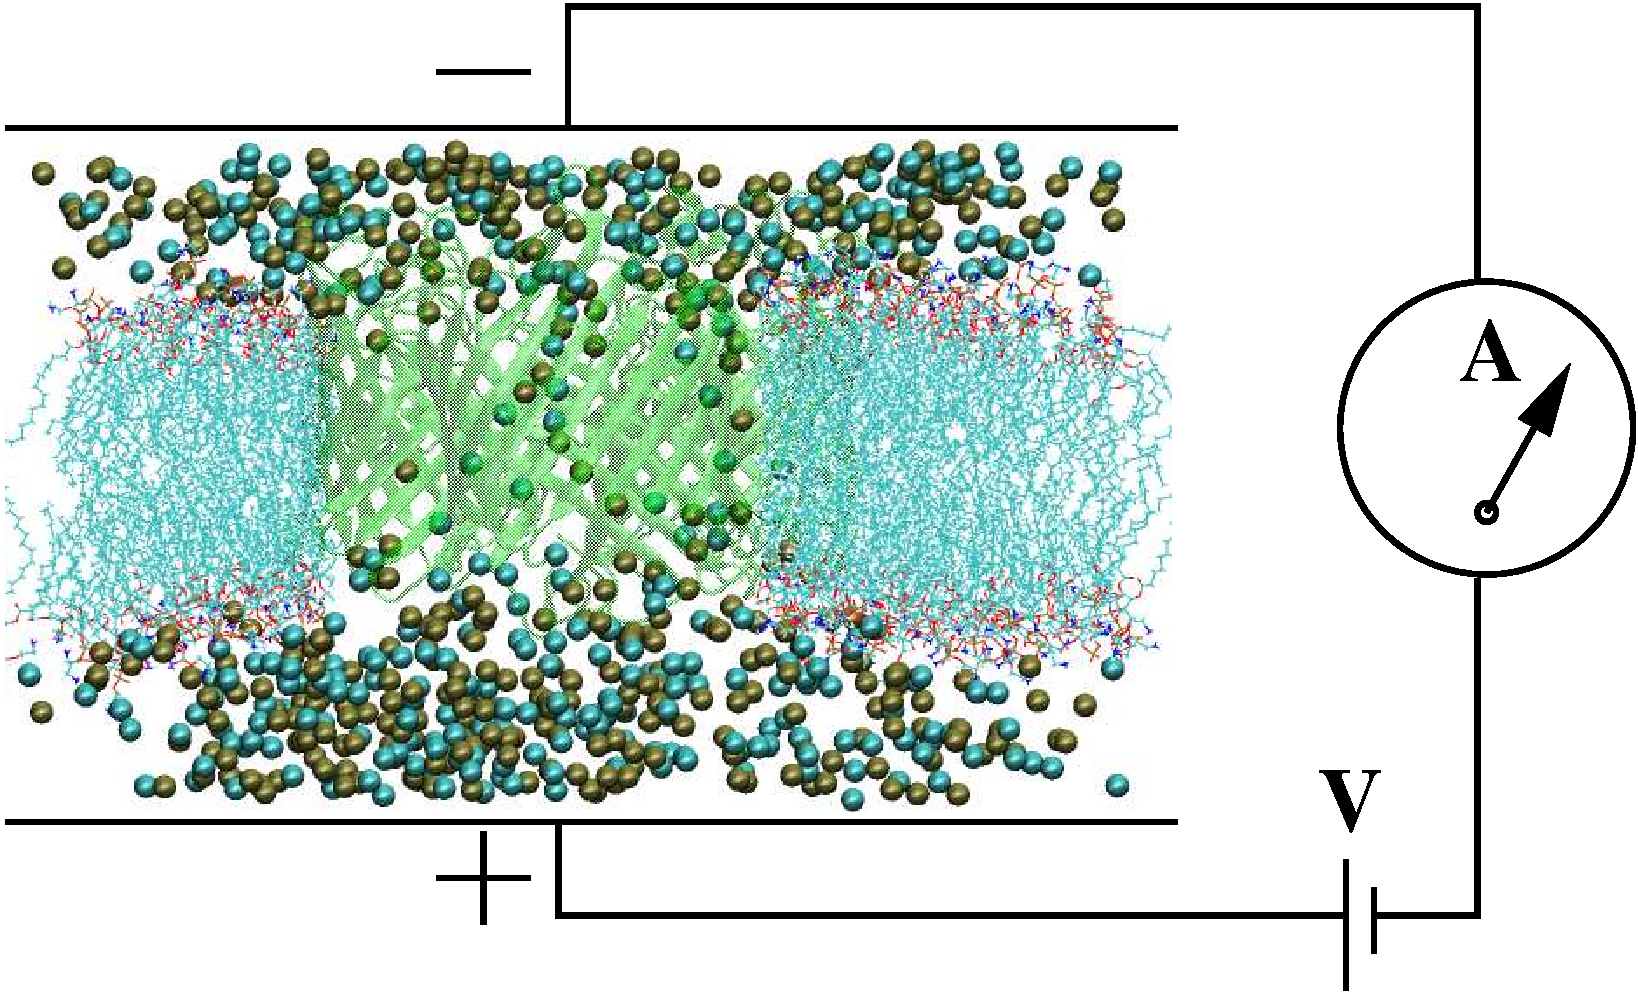
\includegraphics[width=\hsize]{Kleinekathoefer/kleinekathoefer_fig1.pdf}
    \mycaption{Sketch of the ion transport simulations through the OmpF
      protein. A trans-membrane potential is applied to the simulation
      cell.} \label{fig:profkleinekathoefer1}
   \end{center}
\end{figure}

For the simulation and detailed explanation of these experiments a
splitting into two sub-problems is possible: first the determination of the
ion current through the OmpF protein without antibiotics and then in a
second step a steering of the antibiotics through the pore. Within
large-scale molecular dynamics simulation involving about 90 000 atoms a
transmembrane potential is applied. To gain a reasonable statistics the
simulation time needs to be at least 10 ns (1 ns $\approx$ 1 day on 30
2GHz-Opteron-CPUs). Depending on the applied voltage only very few charge
carriers do cross the membrane within 1ns simulation time. Nevertheless the
calculated current and conductivities do correspond rather nicely to the
measured values. Especially the temperature dependence of the ion
conductivity show a similar behavior in experiment and simulations.
First simulations steering substances through the pore also have been
performed. Due to problems with the antibiotics force fields, these test
run had to be done using nucleic acids and sugars. Force fields for
antibiotics are being under development.


\emph{Light-harvesting systems} For an ensemble of B850 rings of the
light-harvesting system LH2 of purple bacteria the linear absorption
spectrum was calculated. Using different Markovian and non-Markovian,
time-dependent and time-independent methods based on second-order
perturbation theory in the coupling between the excitonic system and its
surrounding environment, the influence of the shape of the spectral density
on the linear absorption spectrum was demonstrated for single samples and
in the ensemble average.  For long bath correlation times non-Markovian
effects clearly show up in the static absorption line shapes. Among the
different spectral densities studied was one of the bacterium
\emph{Rhodospirillum (Rs.) molischianum} obtained from molecular dynamics
simulations.  The effect of static disorder on its line shapes in the
ensemble average was analyzed and the results of the present calculations
were compared to experimental data.  \newline \newline Ulrich
Kleinekath\"ofer is also involved in ``Molecular Electronics and Dynamics''.

\myparagraph{Collaborations}
%
Bremen Area Collaborations:
\begin{enumerate}
\item {\sl International University Bremen} \\ Prof. M. Winterhalter
  \\ Ion and antibiotics transport through membrane proteins
  \end{enumerate}
National \& International Collaborations:
\begin{enumerate}
\item {\sl Universit\`a degli Studi di Cagliari} \\ Prof. P. Ruggerone,
  Prof.\ M. Cecarelli
  \\ Transport through membrane proteins
\item {\sl Beckman Institute, University of Illinois at Urbana-Champaign}
  \\ Prof.\ K. Schulten,  B. Isralewitz, PhD
\\ Simulation of a $\beta$-subunit of ATPase
\item {\sl Pittsburgh Supercomputing Center}
  \\ M. Dittrich, PhD \\ Simulation of a $\beta$-subunit of ATPase
\end{enumerate}



\paragraph{Grants}
\begin{enumerate}
\item Funded by DFG, \emph{light-harvesting complexes}, KL
  1299/3-1 (October 2006 - September 2008)
\item Funded by DFG, priority program SPP 1243 \emph{Quantum transport
  at the molecular scale}, KL 1299/4-1 (November 2006 - December
  2008)
\end{enumerate}
\newpage

\nocite{profkleinekathoeferwela05a}
\nocite{profkleinekathoeferschr05a}
\nocite{profkleinekathoeferwela05b}
\nocite{profkleinekathoeferklei06a}
\nocite{profkleinekathoeferklei06b}
\nocite{profkleinekathoeferklei06c}
